%%%%%%%%%%%%%%%%%%%%%%%%%%%%%%%%%%%%%%%%%
% Beamer Presentation
% LaTeX Template
% Version 1.0 (10/11/12)
%
% This template has been downloaded from:
% http://www.LaTeXTemplates.com
%
% License:
% CC BY-NC-SA 3.0 (http://creativecommons.org/licenses/by-nc-sa/3.0/)
%
%%%%%%%%%%%%%%%%%%%%%%%%%%%%%%%%%%%%%%%%%

%----------------------------------------------------------------------------------------
%	PACKAGES AND THEMES
%----------------------------------------------------------------------------------------

\documentclass{beamer}

\mode<presentation> {

% The Beamer class comes with a number of default slide themes
% which change the colors and layouts of slides. Below this is a list
% of all the themes, uncomment each in turn to see what they look like.

%\usetheme{default}
%\usetheme{AnnArbor}
%\usetheme{Antibes}
%\usetheme{Bergen}
%\usetheme{Berkeley}
%\usetheme{Berlin}
%\usetheme{Boadilla}
%\usetheme{CambridgeUS}
%\usetheme{Copenhagen}
%\usetheme{Darmstadt}
%\usetheme{Dresden}
%\usetheme{Frankfurt}
%\usetheme{Goettingen}
%\usetheme{Hannover}
%\usetheme{Ilmenau}
%\usetheme{JuanLesPins}
%\usetheme{Luebeck}
\usetheme{Madrid}
%\usetheme{Malmoe}
%\usetheme{Marburg}
%\usetheme{Montpellier}
%\usetheme{PaloAlto}
%\usetheme{Pittsburgh}
%\usetheme{Rochester}
%\usetheme{Singapore}
%\usetheme{Szeged}
%\usetheme{Warsaw}

% As well as themes, the Beamer class has a number of color themes
% for any slide theme. Uncomment each of these in turn to see how it
% changes the colors of your current slide theme.

%\usecolortheme{albatross}
%\usecolortheme{beaver}
%\usecolortheme{beetle}
%\usecolortheme{crane}
%\usecolortheme{dolphin}
%\usecolortheme{dove}
%\usecolortheme{fly}
%\usecolortheme{lily}
%\usecolortheme{orchid}
%\usecolortheme{rose}
%\usecolortheme{seagull}
\usecolortheme{seahorse}
%\usecolortheme{whale}
%\usecolortheme{wolverine}

%\setbeamertemplate{footline} % To remove the footer line in all slides uncomment this line
%\setbeamertemplate{footline}[page number] % To replace the footer line in all slides with a simple slide count uncomment this line

%\setbeamertemplate{navigation symbols}{} % To remove the navigation symbols from the bottom of all slides uncomment this line
}

\usepackage{graphicx} % Allows including images
\usepackage{booktabs} % Allows the use of \toprule, \midrule and \bottomrule in tables

%----------------------------------------------------------------------------------------
%	TITLE PAGE
%----------------------------------------------------------------------------------------

\title[Journal Club]{Journal club:\\Adjusting for heritable covariates can bias effect in genome-wide association studies } % The short title appears at the bottom of every slide, the full title is only on the title page

\author{Hugues Aschard et al} % Your name
\institute[] % Your institution as it will appear on the bottom of every slide, may be shorthand to save space
{
The American Journal of Human Genetics\\ % Your institution for the title page
\medskip
%\textit{john@smith.com} % Your email address
}
\date{February 5, 2015} % Date, can be changed to a custom date

\begin{document}

\begin{frame}
\titlepage % Print the title page as the first slide
\end{frame}

\begin{frame}
\frametitle{Overview} % Table of contents slide, comment this block out to remove it
\tableofcontents % Throughout your presentation, if you choose to use \section{} and \subsection{} commands, these will automatically be printed on this slide as an overview of your presentation
\end{frame}

%----------------------------------------------------------------------------------------
%	PRESENTATION SLIDES
%----------------------------------------------------------------------------------------

%------------------------------------------------
\section{Introduction} % Sections can be created in order to organize your presentation into discrete blocks, all sections and subsections are automatically printed in the table of contents as an overview of the talk
%------------------------------------------------

\subsection{Context} % A subsection can be created just before a set of slides with a common theme to further break down your presentation into chunks

\begin{frame}
\frametitle{Context}

Heritable human traits have genetic associations.\\\vspace{0.3cm}
Lots of large-scale GWASs published for human traits are adjusted for other correlated traits with a genetic basis. \\
\vspace{0.5cm}
Theoretically:\\
\hspace{0.5cm}Genetic variant can  be associated with both the primary outcome and the covariate used for adjustment.\\\vspace{0.5cm}
So:\\
\hspace{0.5cm}The adjusted and unadjusted estimated effects of the genetic variant on the outcome will differ.\\\vspace{0.5cm}
\textbf{Motivation:} discover genetic variants associated with the primary outcome independently of the correlated trait. \\




\end{frame}

%------------------------------------------------

\begin{frame}
\frametitle{Purpose}
\subsection{Purpose}
Purposes adjustment of covariates in GWASs: 
\begin{itemize}
\item account for potential confounding factors that can bias SNP effect estimates
\item improve statistical power by reducing residual variance
\end{itemize}
\vspace{0.5cm}


Examples: to account for population structure, correlated environmental or demographic factors, to capture batch effects in gene-expression analysis.\\
\vspace{0.5cm}

$\Longrightarrow$ To increase statistical power.\\

\end{frame}


%------------------------------------------------
\begin{frame}
\frametitle{Underlying Causal Diagrams}
\subsection{Underlying Causal Diagrams}
\begin{columns}[c] % The "c" option specifies centered vertical alignment while the "t" option is used for top vertical alignment

\column{.45\textwidth} % Left column and width

\begin{enumerate}
\item genotypes G, 
\item environment E,
\item covariate C,
\item outcome of interest Y.
\end{enumerate}

\column{.8\textwidth} % Right column and width
\begin{figure}
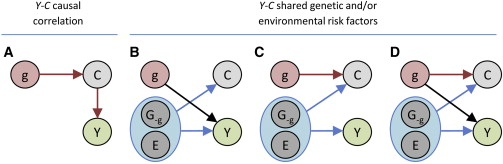
\includegraphics[width=1\linewidth]{fig_1}
\end{figure}

\end{columns}
\end{frame}
%------------------------------------------------
\begin{frame}
\frametitle{Model}
\subsection{Model}
The strength of this association (Fig1C) depends on:

\begin{itemize}
\item $\rho_{CY}$ = Correlation between covariate and outcome due to shared risk factors, \vspace{0.5cm}
\item $\beta_{C}$ = Effect of the genetic variant on the covariate,\vspace{0.5cm}
\item $ \widehat{\beta_{Y}}$ = Bias of the genetic effect estimate (for normalized g, C, and Y with mean 0 and variance 1)\\  \hspace{0.7cm}$\simeq$ $-\beta_{C\rho_{CY}}$ (if $\beta_{C}$ small and sample size sufficiently large). 
\end{itemize}

\end{frame}
%------------------------------------------------
\begin{frame}
\frametitle{Effect Estimates and False Discovery Rate}
\subsection{Effect Estimates and False Discovery Rate}
Product between the direct genetic effect estimate on the covariate and the correlation between the outcome and the covariate.
\begin{columns}[c] % The "c" option specifies centered vertical alignment while the "t" option is used for top vertical alignment

\column{.3\textwidth} % Right column and width
\begin{figure}
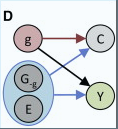
\includegraphics[width=0.5\linewidth]{fig_1_bis}
\end{figure}

\center Increased false discovery rates under the null.

\column{.8\textwidth} % Right column and width
\begin{figure}
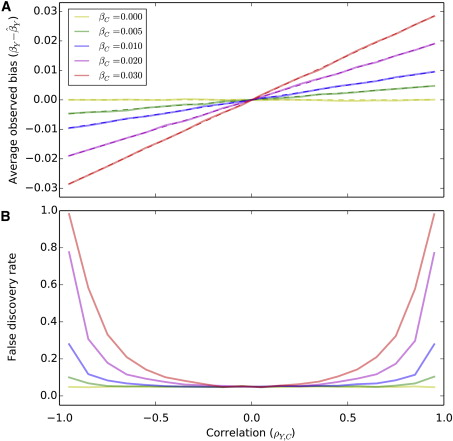
\includegraphics[width=0.7\linewidth]{fig_2}
\end{figure}

\end{columns}
\end{frame}
%------------------------------------------------

\begin{frame}
\frametitle{Potential presence of bias due to adjustment }
\subsection{Potential presence of bias due to adjustment}
\begin{block}{}
Adjusting for covariate with no genetic component \\\hspace{0.5cm}
$\rightarrow$  $\oslash$ bias for genotype effect ($\beta_{C}$ = 0).\\\vspace{0.5cm}
Adjusting for covariate with genetic component ($\beta_{C}$ $\neq$ 0)\\\hspace{0.5cm}
$\rightarrow$ Adjusted association signals difficult to interpret:\\
\begin{itemize}
\item can correspond also to a bivariate signal on Y and C,
\item or to an association with the covariate only. 
\end{itemize}

\end{block}

\end{frame}

%------------------------------------------------

%------------------------------------------------
\section{Illustration}
%------------------------------------------------

\begin{frame}
\frametitle{Illustration}
Examples from published GWAS, 23 SNPs in gender specific samples associated with:\\\hspace{0.3cm}
waist-to-hip ratio(WHR) and waist circumference(WC) adjusted for body mass index (BMI) by Heid et al. and Randal et al.\\\vspace{0.3cm}

Effects on WHR or WC (before/after adjustment for BMI) $+$ Effect BMI \\
\hspace{0.5cm}$\rightarrow$ extracted from the GIANT (statistics database)\\\vspace{0.3cm}

\textbf{Hypothesis:} Genetic effects might be biased as a result of adjustment for body mass index.
 
\end{frame}

%------------------------------------------------
%------------------------------------------------

\begin{frame}
\frametitle{Theory}
\subsection{Theory}
\begin{block}{Theory 1}
The adjusted statistical test can have \textbf{increased power} to detect the genetic variant, as compared to the unadjusted test, if the genetic effect and the phenotypic correlation are in \textbf{opposite directions}. 
\end{block}
\begin{block}{Theory 2}
Conversely, if the genetic effect and the correlation are in the \textbf{same direction}, the adjusted statistical test has, in many cases, a \textbf{decreased power} to detect the genetic variant
\end{block}
\end{frame}

%------------------------------------------------
%------------------------------------------------

\begin{frame}
\frametitle{Simulation}
\subsection{Simulation}
SNPs harboring opposite marginal effects on the two traits are significantly enriched (p = 0.005)\\\vspace{0.3cm}
\textbf{Hypothesis:} Absence of genetic effect on BMI $\rightarrow$ \# SNP with opposite directions of effect follows a binomial distribution (p = 0,5).\\\vspace{0.3cm}
\textbf{Enrichment observed:} A substantial fraction of these SNPs is associated with BMI in the opposite direction.\\\vspace{0.3cm}
$\Rightarrow$ Even non-significant genetic effects on the covariate can influence power when correlation between the outcome and the covariate is large (e.g., ≥ 0.5).
\end{frame}
%------------------------------------------------
\begin{frame}
\frametitle{Heritability of Adjusted Phenotypes}
\subsection{Heritability of Adjusted Phenotypes}
Heritability of a given phenotype VS. Heritability adjusted correlated variable. \\
Upper panel: Heritability variation of Y and C :
\begin{itemize}
\item 0.8 (A), 0.5 (B), 0.2 (C)
\end{itemize}
Bottom panel: Proportion of shared environmental variance from 0 to 1.
\begin{figure}
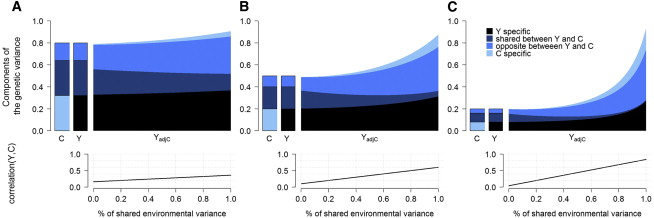
\includegraphics[width=1\linewidth]{fig_3}
\end{figure}

\end{frame}
%------------------------------------------------
%------------------------------------------------
\begin{frame}
\frametitle{Conclusion}
\section{Conclusion}
\begin{block}{}


If purpose of an adjusted analysis is:

\begin{itemize}
\item to increase statistical power rather than detect unbiased direct effects,\\
 $\rightarrow$use multivariate approaches (powerful to detect pleiotropic loci affecting multiple traits)
\item if adjusted analyzes are performed,\\
 $\rightarrow$report estimates of genetic effects on the covariate and pre- and post-adjustment outcomes, their standard deviation and significance, and the correlation between outcome and covariate. 
\end{itemize}
 $\Rightarrow$ The magnitude of a potential bias can be estimated and taken into account when interpreting the results.
\end{block}
\end{frame}

%------------------------------------------------

%------------------------------------------------

\begin{frame}
\Huge{\centerline{Thank you for your attention}}
\end{frame}

%----------------------------------------------------------------------------------------

\end{document}